% Preambule
\documentclass[pdftex,french, english]{article}	% the pdftex is essential

% Packages
% ---
\usepackage[utf8]{inputenc}
\usepackage[T1]{fontenc}
\usepackage[dvips]{graphicx}            % to include images
\usepackage{pslatex}	    % to use PostScript fonts
\usepackage{enumitem}
\usepackage{amsfonts}
\usepackage{babel}
\usepackage{algorithm}
\usepackage[noend]{algpseudocode}
\usepackage[paperwidth=17cm, paperheight=22.5cm, bottom=2.5cm, right=2.5cm]{geometry}
\usepackage{csquotes}
\usepackage{multirow}
\usepackage{caption}
\usepackage{hyperref}

% modifie les parametres de la balise \paragraph

% where to find images:
\graphicspath{{../images/}}

\setcounter{secnumdepth}{4}
\setcounter{tocdepth}{3}
\makeatletter
\newcounter {subsubsubsection}[subsubsection]
\renewcommand\thesubsubsubsection{\thesubsubsection .\@alph\c@subsubsubsection}
\newcommand\subsubsubsection{\@startsection{subsubsubsection}{4}{\z@}%
                                     {-3.25ex\@plus -1ex \@minus -.2ex}%
                                     {1.5ex \@plus .2ex}%
                                     {\normalfont\normalsize\bfseries}}
\newcommand*\l@subsubsubsection{\@dottedtocline{3}{10.0em}{4.1em}}
\newcommand*{\subsubsubsectionmark}[1]{}
\makeatother

\begin{document}
\selectlanguage{english}

\title{INITIATION A LA RECHERCHE}

\begin{titlepage}
\begin{center}

\textsc{\Large Initiation à la recherche}\\[4em]

\begin{figure}[h]
\begin{center}

\includegraphics{lorraine.png}
\end{center}
\end{figure}

\vspace{4em}
\textsc{\Large \textbf{Planification d'actions \\ dans un monde continu}}\\[3em]
\vspace{4em}
\textsc{\textit{Léopold BELLEC, Pierre-Marie JUNGES}}\\[1em]
\vspace{1em}
\textsc{Encadrants : \textit{Olivier BUFFET, Vincent THOMAS}}\\[1em]


\end{center}

\vspace*{\fill}
\textsc{Master 1 Informatique \hspace*{\fill} 2017}

\end{titlepage}

\newpage
\pagenumbering{arabic}

\selectlanguage{french}
\tableofcontents


\newpage
\selectlanguage{english}
\section{Introduction au problème}
	\subsection{Problèmatique}
	Une des problématiques importantes en intelligence artificielle est la planification automatique d’actions, que ce soit pour la robotique, pour les jeux (échecs, go, ...), pour la gestion de sources d’énergie, ou pour la protection d’espèces menacées. La plupart des algorithmes développés n’abordent que des situations dans lesquelles le nombre d’états (le nombre de situations) possibles est fini et relativement petit, tout comme le nombre d’actions disponibles. Ces limitations viennent de ce que ces algorithmes raisonnent sur l’arbre des évolutions possible du “système” à contrôler, arbre dont la taille subit une explosion combinatoire avec les nombres d’états et d’actions (et qui n’a plus de sens quand les facteurs de branchement sont infinis).
	\subsection{Pourquoi ce sujet ?}
	Nous avions étudié lors de l'UE \textit{Modèles de perception, de raisonnement et d’interaction} l'algorithme \textbf{M}onte \textbf{C}arlo \textbf{T}ree \textbf{S}earch \cite{coulom01} appliqué au jeu Puissance $4$. 

	Or cette application était dans un espace où les états et actions possibles étaient finis, et au vue des parties effectuées contre cet algorithme il était difficile voir impossible de le battre. 

	C'est pourquoi, nous avons souhaité pousser un peu plus nos connaissances sur cet algorithme et surtout étudier ses performances dans un espace qui serait maintenant continu (une infinitée d'actions ou états possibles) soit un espace proche de la réalité, proche du comportement humain. 

	De plus, ce sujet est peu étudié ce qui le rend encore plus intéressant.
	
	\subsection{Notre approche}
	Étant donné le nombre imposant d'états ou d'actions possibles à chaque étape, nous avons donc tout simplement essayer à chaque étape de réduire ce nombre de choix possible jusqu'à avoir un espace plus restreint \cite{couetoux01}.

	C'est donc cette solution que nous avons choisie pour répondre à cette problèmatique. 

	Afin de pouvoir mettre en place l'algorithme, nous avions deux choix d'implémentations, utiliser le langage C ou bien le langage Java. Notre choix s'est finalement porté sur le langage Java.
\newpage





\section{Le B.A.-BA de l'algorithme MCTS}
	\subsection{Les bases du Monte Carlo Tree Search}
	\subsubsection{Définition}
	Monte Carlo Tree Search ou bien MCTS est un algorithme de recherche, qui, à partir d'un noeud initial $n_{i}$ indique la meilleure action $a_i$ à utiliser afin d'atteindre un noeud intermédiaire $n_{int}$ proche du noeud terminal recherché $n_{t}$. 

	L'application de méthodes de Monte Carlo fait appel à de nombreuses simulations, cela veut donc dire que lors du déroulement de l'algorithme, un certain nombre d'actions seront joués de manière aléatoire.
	\subsubsection{Déroulement de l'algorithme}
	L'algorithme est exécuté tant que le temps limite $t$ n'est pas écoulé, et se décompose en 4 étapes :
	\begin{figure}[h]
		\centering
		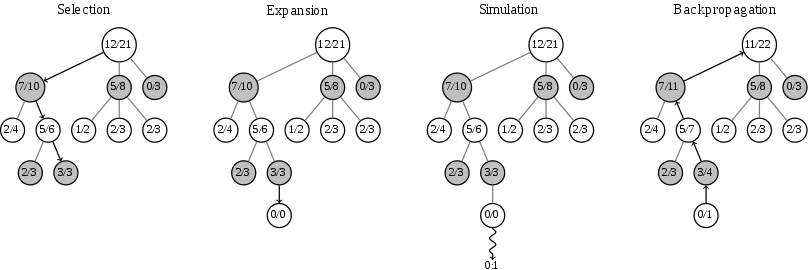
\includegraphics[width=\textwidth]{etapes.png}
		\caption{ Étapes de MCTS}
		 \label{fig:mcts}
	\end{figure}

\textit{Notation : Le noeud correspond à un état du jeu et (12/21) signifie 12 victoires sur 21 simulations.} 
	\begin{enumerate}
		\item \textbf{Sélection}

		À cette étape, l'algorithme va sélectionner parmis ses noeuds suivants le noeud avec la plus grande valeur selon la formule de sélection utilisée (voir section 2.2). 

		Dans la figure~\ref{fig:mcts}, on s'aperçoit que l'algorithme sélectionne à tour de rôle le noeud $(7/10)$, puis le noeud $(5/6)$ et enfin le noeud $(3/3)$ et s'arrête car ce noeud n'est pas développé.
		\item \textbf{Expension}

		Une fois le meilleur noeud sélectionné, cet étape va lui rajouté un ou plusieurs noeud enfants, accessible en faisant 1 seule action à partir du noeud courant. 

		Dans la figure~\ref{fig:mcts}, l'algorithme rajoute au noeud courant $(3/3)$ le noeud enfant $(0/0)$.
		\item \textbf{Simulation}

		Maintenant qu'un nouveau noeud a été ajouté, l'algorithme va jouer aléatoirement jusqu'à atteindre un noeud qualifié de terminal.
		C'est dans cette partie qu'on utilise le principe Monte Carlo, c'est-à-dire l'utilisation de l'aléatoire.
		\item \textbf{Mise à jour} 

		L'algorithme a atteint un noeud terminal, il faut donc récupérer sa récompense (par exemple +1 si c'est un noeud gagnant 0 sinon). Puis faire remonter cette récompense jusqu'au noeud racine et mettre à jour les statistiques. 

		Dans la figure~\ref{fig:mcts} ci-dessus le noeud terminal était donc perdant car $(0/1)$, donc on va augmenter uniquement le nombre de simulation de chacun de ces noeuds, d'où la transformation du noeud $(3/3)$ en $(3/4)$ par exemple.
	\end{enumerate}
	\subsubsection{Pseudo-code}
	\begin{algorithm}
	\caption{MCTS générique}
	  \label{alg:mcts}
	\begin{algorithmic}[1]
	\Function{MCTS}{État $s$}
	\State création d'un noeud $n$ à partir de $s$
	\While{$temps < tempsLimite $}\Comment{tant qu'il reste du temps}
	\State $n \gets selection(n)$ \Comment{L'étape d'expension est incluse dans cet appel}
	\State $n \gets simulation(n)$
	\State $n \gets miseAjour(n)$
	\EndWhile
	\State \textbf{return} $meilleurEnfant(n)$
	\EndFunction
	\end{algorithmic}
	\end{algorithm}
    
    
    
    
    
	\subsection{Formule de sélection utilisée}
	Précédemment, nous avions parlé lors de l'étape de sélection, de formule de sélection. 

	En effet, afin de choisir le meilleur noeud possible des formules ont été mise en place.

	C'est dans cette partie que nous allons en expliquer une, de nouvelles formules de sélection seront introduites
	dans la section suivante.


	\textit{Notation : Soit $n$ un noeud, $N$ son noeud parent, et C une constante d'exploration.} 

	\begin{enumerate}
		\item Upper Confidence Bounds (\textbf{UCB}) \\
		\[ \frac{recompenses(n)}{simulations(n)} + C \times \sqrt{\frac{simulations(N)}{simulations(n)}} \] 

		On se rend compte ici que si notre constante \textit{C} est égale à $0$ alors, l'algorithme va choisir le noeud $n$ avec le meilleur rapport $\frac{recompenses(n)}{simulations(n)}$ possible. 

		Donc si l'on souhaite permettre une exploration de l'arbre, il faut que $C$ soit différent de $0$ sinon on voit bien que si à l'état initiale l'algorithme sélectionne un noeud $n$, alors ce dernier aura nécessaire le meilleur rapport $\frac{recompenses(n)}{simulations(n)}$ vu qu'il est le seul à avoir été développé, et donc il sera tout au long de l'algorithme choisit. 

		De ce fait, la constante d'exploration $C$ est donc fixé à $\sqrt{2}$ afin de permettre de développer l'arbre de recherche.


		\underline{\textbf{Lexique}} : On utilise le terme UCT (\textit{Upper Confidence Bound for Trees}) pour désigner l'algorithme MCTS utilisant une formule de sélection de type UCB.
	\end{enumerate}





	\subsection{Stratégies de sélection terminale}
	Les formules explicitées ci-dessus ont pour rôle de choisir le meilleur enfant lorsque l'algorithme se trouve à l'étape de sélection. 

	Dans cette partie, l'algorithme est terminé et l'arbre a été développé. Nous ne pouvons donc plus réutiliser les formules précèdentes car la constante d'exploration \textit{C} n'a plus de sens ici. 

Il faut donc trouver d'autres moyens pour choisir le meilleur noeud enfant. 
Cette étape correspond à l'appel \textit{meilleurEnfant(n)} dans l'algorithme~\ref{alg:mcts}. 
Or, nous savons qu'un noeud $n$ possède un nombre de simulation, et de récompense.
	À partir de ces deux informations nous avons utilisé 3 stratégies de sélection :
	\begin{enumerate}
		\item Robuste :
		
		On choisit le noeud avec le plus grand nombre de simulation.
		\item Maxi :  
		
		On choisit le noeud qui possède la valeur de récompense la plus élevée.
		\item Maxi-Robuste :
		
		On choisit le noeud ayant le meilleur rapport $\frac{recompense}{simulation}$.
	\end{enumerate}
    
    
    
    
    
	\subsection{Application sur un exemple}
	Maintenant que nous avons vu comment l'algorithme fonctionnait de manière générale, nous l'avons mis en pratique sur le jeu du type Puissance $4$. 
    

    Pour rappel voici la règle du jeu selon wikipedia\footnote{\url{https://fr.wikipedia.org/wiki/Puissance_4}} :
   
    \begin{displayquote}
    \textit{``Le but du jeu est d'aligner 4 pions sur une grille comptant 6 rangées et 7 colonnes. Chaque joueur dispose de 21 pions d'une couleur (par convention, en général jaune ou rouge). Tour à tour les deux joueurs placent un pion dans la colonne de leur choix, le pion coulisse alors jusqu'à la position la plus basse possible dans la dite colonne à la suite de quoi c'est à l'adversaire de jouer. Le vainqueur est le joueur qui réalise le premier un alignement (horizontal, vertical ou diagonal) d'au moins quatre pions de sa couleur. Si, alors que toutes les cases de la grille de jeu sont remplies, aucun des deux joueurs n'a réalisé un tel alignement, la partie est déclarée nulle.''}
   	\end{displayquote}


	Après de nombreux essais, humain contre ordinateur, nous avons remarqué qu'il était très compliqué voir impossible de battre l'algorithme à partir d'un certain temps $t$, et sur un ordinateur avec un processeur type $i7$ ce temps est d'environ $2$ secondes.
	

Afin de poursuivre un peu plus notre expérience, nous avons décidé de faire jouer $2$ ordinateurs l'un contre l'autre, et, de cette facon, comparer les différentes stratégies de sélection finales et voir si effectivement certaines sont plus efficaces que d'autres.
		\\
		\begin{table}[h]
		\begin{tabular}{cc|c|c|c|c}
			\cline{3-5}
			& & \multicolumn{3}{ c| }{Ordinateur 2} \\ \cline{3-5}
			& & Robuste & Maxi & Robuste-Maxi \\ \cline{1-5}
			\multicolumn{1}{ |c  }{\multirow{3}{*}{Ordinateur 1} } &
			\multicolumn{1}{ |c| }{Robuste} & 70-30-0 & 60-40-0 & 60-40-0 &    \\ \cline{2-5}
			\multicolumn{1}{ |c  }{}                        &
			\multicolumn{1}{ |c| }{Maxi} & 80-20-0 & 80-20-0 & 50-50-0 &     \\ \cline{2-5}
			\multicolumn{1}{ |c  }{}                        &
			\multicolumn{1}{ |c| }{Maxi-Robuste} & 90-10-0 & 60-40-0 & 70-30-0 &     \\ \cline{1-5}
		\end{tabular}
			\caption{Comparatif des différentes stratégies}\label{tabular:compa}
		\end{table}

\underline{\textit{Méthodes expérimentales et explications de la table~\ref{tabular:compa}}} : 
\\ \\
L'ordinateur 1 commence \textbf{toujours} les parties, la notation $x-y-z$ signifie $x\%$ de victoire(s) pour l'ordinateur 1, $y\%$ de victoire(s) pour l'ordinateur 2, $z\%$ de match(s) nul(s).

Comme nous pouvons le remarquer, l'ordinateur commencant la partie à globalement plus de chance de gagner, peu importe la stratégie utilisée.


Réfléchissons sur la stratégie Maxi, dans le jeu Puissance $4$ nous avons fixé la récompense en cas de victoire à $1$ peu importe si la victoire était "serrée" ou bien "écrasante". 

Or plaçons nous maintenant dans le cas où nous aurions fait des récompenses différentes selon le type de victoire, posons par exemple $1$ par une victoire "serrée" et $10$ pour une victoire "écrasante". 

De ce fait, si nous avions un noeud avec $19$ de récompense décomposé en $19$ victoires dites "serrées" et $1$ défaite, et un autre noeud avec $20$ de récompense mais composée seulement de $2$ victoires "écrantes" et $18$ défaites.
Alors dans ce cas, la stratégie Maxi nous retournera le noeud avec $20$ de récompense alors que nous aurions pu prendre le noeud qui a $19$ victoires sur $20$ simulations et qui est donc plus intéressant car son pourcentage de victoire est plus élévé.

Donc, pour pouvoir utiliser la stratégie Maxi de manière efficace, il est préférable de l'utiliser sur un jeu où l'on a une unique récompense en cas de victoire (ce qui est le cas du Puissance $4$).
\\ \\
Utilisons maintenant ce même raisonnement ainsi que ce même cas de figure pour la stratégie Robuste, nous avons donc $2$ noeuds avec $20$ simulations chacuns. 

Or on est censé choisir le noeud ayant le maximum de simulations possible, donc notre stratégie Robuste va tout simplement retourner le premier noeud lu car le deuxième noeud lu n'aura pas un nombre de simulation strictement supérieur au premier noeud. Alors, dans notre cas de figure, la stratégie Robuste aura une probabilité de $\frac{1}{2}$ de retourner le meilleur noeud (celui avec les $19$ victoires).

Donc, de la même façon que la stratégie Maxi, la stratégie Robuste n'est pas nécessairement bonne pour choisir le meilleur noeud possible.
\\ \\
À partir des raisonnements ci-dessus il est donc facile de se convaincre que choisir la stratégie Maxi-Robuste est préférable, car le fait qu'elle prenne le meilleur rapport $\frac{recompense}{simulation}$ l'empêche donc d'être biaisé, car son choix dépend donc de 2 critères.
\\ \\
Maintenant que nous savons comment MCTS fonctionne dans un monde avec un nombre d'états et d'actions discret, essayons de le mettre en pratique dans un monde à actions ou états continue.

\newpage
\section{Application dans un monde continue}
\subsection{Abstrait}
	\subsubsection{Définitions}
	\subsubsection{Contexte}
	\subsubsection{Première approche}
		\subsubsubsection{Modification du MCTS discret}
	\subsubsection{Progressive widening}
	\subsubsection{Double peogressive widening}
\subsection{Expérimentations}
	\subsubsection{MCTS discret dans un monde continu}
	\subsubsection{Progressive widening}
		\subsubsubsection{Sans ajout de bruit}
		\subsubsubsection{Avec ajout de bruit}
	\subsubsection{Double progressive widening}
\subsection{Conclusion}
\newpage
\selectlanguage{french}
\bibliographystyle{alpha}
\bibliography{biblio.bib}

\end{document}